% TODO: Falar sobre a infraestrutura cloud do front-end

% TODO!: FALAR SOBRE AS MULTIPLAS REGIÕES GEOGRÁFICAS

% TODO: Revisar com GPTero

\section{Infraestrutura Cloud}
% TODO: Explicar sobre o que será abordado nesse capítulo

Neste capítulo, será apresentada a infraestrutura em nuvem utilizada para hospedar a plataforma Codeboard. Serão abordados os serviços de computação, banco de dados, controle de acesso, segurança, balanceamento de carga, escalabilidade, monitoramento, logs, gestão de incidentes, recuperação de desastres, entre outros. 

A infraestrutura foi projetada para ser altamente disponível, com redundância em todas as camadas, de modo que a plataforma Codeboard possa suportar um grande número de usuários simultâneos sem interrupções. Além disso, a infraestrutura foi projetada para ser escalável, de modo que possa crescer ou diminuir de acordo com a demanda, sem a necessidade de intervenção manual.

\subsection{Visão Geral da Arquitetura Utilizada}
% TODO: Rever

Para garantir a alta disponibilidade e escalabilidade da plataforma Codeboard, a infraestrutura em nuvem do backend foi projetada para seguir o modelo \emph{Multi-Region Active-Active}\ref{multi-region-aa}, onde a aplicação é distribuída em várias regiões geográficas, de modo que, em caso de falha em uma região, o tráfego seja automaticamente redirecionado para outra região. A arquitetura em nuvem da plataforma Codeboard é composta por várias camadas, cada uma com um conjunto específico de serviços e funcionalidades. A Figura \ref{fig:cloud-architecture} demonstra a visão geral da arquitetura em nuvem da plataforma Codeboard. 

\begin{figure}[H]
    \centering
    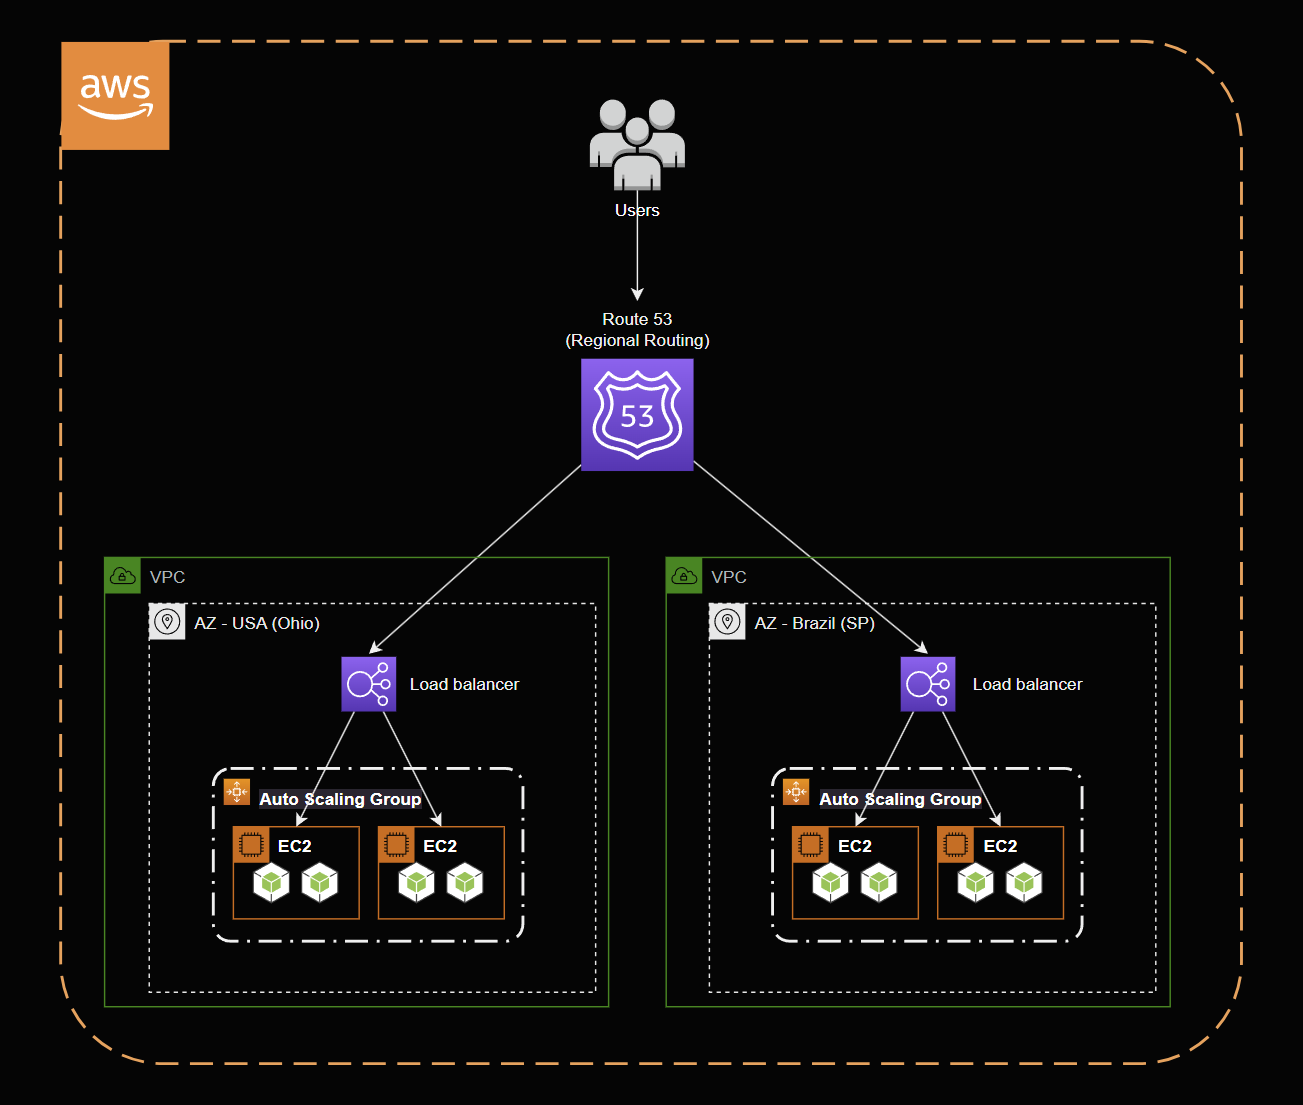
\includegraphics[width=\textwidth]{drawio/cloud-architecture.png}
    \caption{Visão Geral da Arquitetura em Nuvem}
    \label{fig:cloud-architecture}
\end{figure}


\subsubsection{Planejamento de Infraestrutura}
% TODO: Linkar melhor com active-active? Justificar sua escolha
% Revisado

O planejamento da infraestrutura da plataforma começou com a definição de requisitos e necessidades específicas da aplicação, que incluem:

\begin{itemize}
    \item \textbf{Baixa latência}: Para assegurar uma experiência de usuário fluida e responsiva em tempo real, a plataforma Codeboard precisa operar com baixa latência.
    \item \textbf{Alta disponibilidade}: Codeboard deve estar acessível 24/7, garantindo operação contínua, mesmo durante atualizações e manutenções.
    \item \textbf{Escalabilidade}: A plataforma deve suportar um grande número de usuários simultâneos, aumentando ou diminuindo seus recursos conforme a demanda.
    \item \textbf{Resiliência}: Codeboard precisa de mecanismos de recuperação automática frente a falhas de hardware ou software, sem impacto na experiência do usuário.
    \item \textbf{Custo-efetividade}: A infraestrutura deve ser otimizada para minimizar custos, evitando ociosidade de recursos.
    \item \textbf{Facilidade de gerenciamento}: a infraestrutura deve ser simples de gerenciar, utilizando práticas de DevOps, como \emph{Infra-as-Code} (IaC) e \emph{Continuous Integration/Continuous Deployment} (CI/CD). % TODO: Abordar mais sobre a implantação da infraestrutura como código
    \item \textbf{Segurança}: A plataforma deve ser protegida contra ameaças e ataques cibernéticos.
    \item \textbf{Monitoramento}: A plataforma deve contar com métricas e logs para acompanhar desempenho e integridade.
\end{itemize}

A plataforma Codeboard foi hospedada na Amazon Web Services (AWS), uma escolha estratégica baseada em fatores como a ampla variedade de serviços, escalabilidade, confiabilidade e presença global de data centers. Utilizando a AWS, a Codeboard se beneficia de recursos essenciais para sua operação, como computação, armazenamento, banco de dados, redes, segurança e monitoramento. A infraestrutura global da AWS permite distribuir a aplicação em várias regiões, garantindo alta disponibilidade e baixa latência para os usuários. Além disso, o \emph{free tier} da AWS foi um diferencial importante, possibilitando o desenvolvimento e os testes iniciais sem custos significativos.

Para atender a esses requisitos, foram escolhidos os seguintes serviços da AWS para compor a infraestrutura da plataforma Codeboard:

\begin{itemize}
    \item \textbf{Amazon Elastic Compute Cloud (EC2)}: Fornece instâncias virtuais escaláveis e seguras para execução da aplicação.
    \item \textbf{Amazon Elastic Load Balancing (ELB)}: Distribui o tráfego entre instâncias EC2, garantindo alta disponibilidade e escalabilidade.
    \item \textbf{AWS Auto Scaling}: Ajusta automaticamente a capacidade das instâncias EC2 conforme a demanda.
    % \item \textbf{Amazon DocumentDB}: serviço de banco de dados NoSQL que fornece instâncias gerenciadas de bancos de dados MongoDB.
    % \item \textbf{Amazon ElastiCache}: serviço de cache em memória que fornece instâncias gerenciadas de Redis.
    \item \textbf{Amazon Virtual Private Cloud (VPC)}: Cria uma rede virtual com sub-redes privadas, gateways de internet e regras de firewall.
    \item \textbf{Amazon Route 53}: Configura registros de DNS, oferece balanceamento de carga entre regiões geográficas e failover.
    \item \textbf{Amazon CloudWatch}: Proporciona métricas, logs e alarmes para monitorar a saúde e o desempenho da aplicação.
    \item \textbf{AWS Identity and Access Management (IAM)}: Gerencia o controle de acesso, permitindo a criação de usuários, grupos e políticas.
    \item \textbf{AWS Certificate Manager (ACM)}: Facilita a criação, renovação e implantação de certificados SSL/TLS para segurança de dados.
\end{itemize}

Essas escolhas de serviço atendem diretamente às necessidades de desempenho, segurança e custo, alinhando a infraestrutura às metas de alta disponibilidade e resiliência exigidas pela plataforma.


\subsection{Infraestrutura de Computação}

Tendo em vista que será utilizado o modelo \emph{Multi-Region Active-Active}, a infraestrutura de computação da plataforma Codeboard foi projetada para ser distribuída em várias regiões geográficas da AWS, de modo que, em caso de falha em uma região, o tráfego seja automaticamente redirecionado para outra região. A infraestrutura de computação é composta por instâncias EC2, balanceamento de carga, escalabilidade automática, controle de acesso e segurança, monitoramento, logs, gestão de incidentes, recuperação de desastres, entre outros.

\subsubsection{Servidor Virtual}
% Revisado

Para hospedar a aplicação da plataforma Codeboard, foram escolhidas instâncias EC2 do tipo \emph{t3.micro}, adequadas ao estudo de caso pelos seguintes motivos: 

\begin{itemize}
    \item \textbf{Custo}: As instâncias t3.micro fazem parte do \emph{free tier} da AWS, oferecendo 12 meses de uso gratuito, o que torna essa opção financeiramente viável para a fase inicial do projeto.
    \item \textbf{Desempenho Escalável}: Com capacidade de burst, essas instâncias podem fornecer recursos adicionais de CPU temporariamente, sem custos extras, atendendo a picos de demanda.
    \item \textbf{2 vCPUs}: As instâncias t3.micro possuem 2 vCPUs, que é o mínimo recomendado para a aplicação da plataforma Codeboard, que opera em um \emph{cluster} de processos, onde cada processo é uma aplicação Node.js que é responsável pelo backend.
    \item \textbf{1 GB de memória RAM}: A memória de 1 GB é adequada para a Codeboard, pois sua função de intermediação de mensagens em tempo real requer um baixo consumo de memória.
    \item \textbf{Armazenamento em disco SSD}: Embora a Codeboard não faça uso intensivo de disco, o armazenamento SSD nas instâncias t3.micro oferece maior velocidade e confiabilidade, beneficiando a estabilidade do sistema.
\end{itemize}

As instâncias EC2 foram configuradas com o sistema operacional \emph{Ubuntu 24.04 LTS}, o servidor web \emph{NGINX}, o gerenciador de processos \emph{PM2} e entre outras ferramentas. A escolha do Ubuntu 24.04 LTS deve-se à sua estabilidade e suporte de longo prazo para atualizações de segurança. O NGINX atua como um servidor web reverso, redirecionando o tráfego HTTPS para os processos Node.js que executam a Codeboard. Já o PM2 gerencia esses processos, mantendo-os ativos e reiniciando automaticamente em caso de falhas.

\subsection{Balanceamento de Carga, Escalabilidade e Recuperação de Falhas}
% Revisado

A arquitetura da plataforma Codeboard foi projetada com uma estratégia de balanceamento de carga, escalabilidade e recuperação de falhas que abrange múltiplos níveis de operação, assegurando alta disponibilidade, baixa latência e resiliência. Esta seção apresenta a abordagem utilizada para distribuir de forma eficiente o tráfego e garantir que a aplicação responda de maneira otimizada, mesmo em cenários de alta demanda ou falhas inesperadas.

Em primeiro lugar, o balanceamento de carga entre processos permite uma distribuição equitativa das requisições entre processos individuais da aplicação, garantindo o uso eficiente dos recursos da instância. Para lidar com o tráfego em servidores múltiplos, foi configurado um segundo nível de balanceamento de carga que distribui as requisições entre instâncias EC2 da AWS, de modo que a aplicação possa escalar horizontalmente conforme a demanda. Por fim, para maximizar a disponibilidade global e reduzir a latência para usuários em diferentes localidades, foi implementado um balanceamento de carga geográfico entre regiões da AWS, utilizando o Route 53 para redirecionar o tráfego para a região mais próxima do usuário.

Além disso, mecanismos de recuperação automática de falhas foram configurados em cada nível. Esses mecanismos monitoram continuamente a saúde dos processos e das instâncias, substituindo automaticamente recursos que falhem e garantindo a continuidade da aplicação. Essa estrutura multissetorial de balanceamento e recuperação permite que a plataforma Codeboard mantenha uma operação robusta e confiável, capaz de lidar com flutuações de carga e com interrupções inesperadas.

\subsubsection{Balanceamento de Carga entre Processos}
% Revisado

A aplicação Codeboard opera em um \emph{cluster} de processos, o que torna o balanceamento de carga essencial para distribuir o tráfego de entrada de maneira eficiente. Para isso, o PM2 foi configurado no modo cluster, permitindo a criação de múltiplos processos Node.js que compartilham o mesmo \emph{socket} de rede. Dessa forma, o NGINX redireciona o tráfego entre os processos por meio do módulo \emph{proxy\_pass}, que envia as requisições HTTP para o processo Node.js que executa a Codeboard.

O algoritimo de balanceamento de carga utilizado é o \emph{Round Robin}, que distribui o tráfego de entrada de forma alternada entre os processos do cluster, assegurando que cada processo receba uma quantidade igual de solicitações. A Figura \ref{fig:round-robin-load-balancing} ilustra o funcionamento do algoritmo Round Robin, enqunato a Figura \ref{fig:pm2-cluster-mode} mostra o modo cluster do PM2 em ação.

\begin{figure}[H]
    \centering
    \includegraphics[width=\textwidth]{diagrams/round-robin-load-balancing.png}
    \caption{Balanceamento de Carga com Round Robin}
    \label{fig:round-robin-load-balancing}
\end{figure} 

\begin{figure}[H]
    \centering
    \includegraphics[width=\textwidth]{diagrams/pm2-cluster-mode.png}
    \caption{Modo Cluster do PM2}
    \label{fig:pm2-cluster-mode}
\end{figure}

O balanceamento de carga entre processos otimiza o uso dos recursos de CPU e memória, distribuindo a carga de trabalho de maneira uniforme entre os vCPUs das instâncias EC2, garantindo um desempenho estável e eficiente.

\subsubsection{Recuperação Automática de Falhas em Processos}
% Revisado

O balanceamento de carga entre processos também contribui para a alta disponibilidade e confiabilidade da aplicação. Em caso de falha de um dos processos, o tráfego é automaticamente redirecionado para outros, evitando interrupções para os usuários.

Para reforçar a tolerância a falhas e garantir a alta disponibilidade, foram configurados no PM2 mecanismos de monitoramento e recuperação automática. Esse monitoramento verifica continuamente os processos Node.js e, ao detectar uma falha, reinicia o processo comprometido. A Figura\ref{fig:pm2-fault-tolerance} ilustra o funcionamento do monitoramento e recuperação de falhas pelo PM2, garantindo que a aplicação permaneça em funcionamento mesmo diante de falhas pontuais.


\begin{figure}[H]
    \centering
    \includegraphics[width=0.75\textwidth]{diagrams/pm2-fault-tolerance.png}
    \caption{Tolerância à Falhas com PM2}
    \label{fig:pm2-fault-tolerance}
\end{figure}


\subsubsection{Balanceamento de Carga entre os Servidores}
% Revisado

A infraestrutura de computação da plataforma Codeboard foi projetada para ser distribuída e redundante, assegurando que o tráfego seja balanceado entre várias instâncias EC2 e entre diferentes regiões geográficas. Para essa finalidade, utilizou-se o AWS Elastic Load Balancing (ELB), que distribui o tráfego de entrada de forma equilibrada entre as instâncias, garantindo alta disponibilidade e escalabilidade da aplicação.

Entre os tipos de ELB disponíveis, como o Application Load Balancer (ALB), Network Load Balancer (NLB) e Classic Load Balancer (CLB), escolheu-se o ALB. Esse balanceador de camada 7 permite o roteamento de tráfego com base em critérios específicos, como URL, cabeçalhos HTTP e métodos HTTP. O ALB foi configurado com um certificado SSL para assegurar a segurança do tráfego HTTPS entre clientes e servidores.

O algoritmo de balanceamento de carga adotado foi o \emph{Round Robin}, que distribui o tráfego de forma equitativa entre as instâncias EC2, garantindo uma divisão equilibrada de requisições.


% TODO: Voltar no capítulo 3 para explicar a importância do Health Check? Testar se a conexão com o banco de dados está funcionando, se a aplicação está respondendo, etc.

Para garantir que apenas instâncias saudáveis recebam tráfego, foram configurados \emph{Health Checks} para monitorar a saúde das instâncias EC2. Os Health Checks realizam verificações periódicas em uma rota específica da aplicação Codeboard, permitindo que o ELB detecte se cada instância está respondendo corretamente. Se uma instância não responder adequadamente ao Health Check, o ELB a marca como indisponível e redireciona o tráfego para outras instâncias saudáveis.

Configurou-se o Health Check com um intervalo de 30 segundos e um tempo limite de 5 segundos, o que significa que o ELB realiza uma verificação a cada 30 segundos e aguarda uma resposta dentro de 5 segundos. Após duas falhas consecutivas, a instância é marcada como indisponível e o tráfego é redirecionado para outras instâncias saudáveis. A Figura \ref{fig:elb-health-check} ilustra o funcionamento do Health Check do ELB.

\begin{figure}[H]
    \centering
    \includegraphics[width=0.75\textwidth]{diagrams/elb-health-check.png}
    \caption{Health Check do ELB}
    \label{fig:elb-health-check}
\end{figure}


\subsubsection{Escalabilidade Horizontal com Auto Scaling}
% Revisado

Para garantir a alta disponibilidade da plataforma Codeboard, a infraestrutura foi projetada para escalar horizontalmente, permitindo que a aplicação aumente ou reduza seus recursos de acordo com a demanda, sem necessidade de intervenção manual. Essa escalabilidade automática foi implementada com o AWS Auto Scaling, que ajusta a quantidade de instâncias EC2 com base na utilização de recursos.

O Auto Scaling utiliza um Auto Scaling Group (ASG) para monitorar a utilização de CPU nas instâncias EC2 e ajustar a quantidade de instâncias conforme uma política de escalabilidade. Definiram-se gatilhos específicos: quando a utilização de CPU ultrapassa um limite predefinido, uma nova instância é adicionada ao grupo, distribuindo melhor a carga. Inversamente, se a utilização de CPU cair abaixo de um limite, o ASG reduz o número de instâncias, otimizando custos. Foi configurado um número mínimo e máximo de instâncias, garantindo um custo controlado e uma capacidade mínima sempre disponível. A Figura \ref{fig:auto-scaling-horizontal-scalability} ilustra essa escalabilidade horizontal com o Auto Scaling.

\begin{figure}[H]
    \centering
    \includegraphics[width=\textwidth]{diagrams/auto-scaling-horizontal-scalability.png}
    \caption{Escalabilidade Horizontal com Auto Scaling Group}
    \label{fig:auto-scaling-horizontal-scalability}
\end{figure}

Os limites de gatilhos de escalabilidade foram definidos com base em testes e monitoramento da aplicação, estabelecendo 70\% de uso de CPU para adicionar uma nova instância e 30\% para removê-la. Os valores de instâncias mínima e máxima foram configurados entre 1 e 5, podendo ser ajustáveis conforme previsões de tráfego, sazonalidade e eventos especiais.

\subsubsection{Recuperação Automática de Falhas em Servidores}
% Revisado

O Auto Scaling do AWS também possui um mecanismo de recuperação automática de falhas, que monitora continuamente a saúde das instâncias EC2. Quando uma instância é marcada como indisponível pelo ELB (por falhar em um Health Check), o Auto Scaling substitui automaticamente a instância defeituosa por uma nova, garantindo que a aplicação da plataforma Codeboard permaneça sempre disponível e resiliente a falhas. Essa combinação de Auto Scaling, ELB e PM2 resulta em uma arquitetura altamente disponível, escalável e confiável. A Figura \ref{fig:auto-scaling-fault-tolerance} ilustra o funcionamento da recuperação automática de falhas com o Auto Scaling.

\begin{figure}[H]
    \centering
    \includegraphics[width=\textwidth]{diagrams/auto-scaling-fault-tolerance.png}
    \caption{Recuperação Automática de Falhas com Auto Scaling}
    \label{fig:auto-scaling-fault-tolerance}
\end{figure}

Durante a inicialização de uma nova instância, o Auto Scaling aplica um \emph{warmup time} de 180 segundos, período necessário para que a instância esteja completamente operacional. Nesse tempo, são realizadas tarefas como configuração da instância, inicialização da aplicação e estabelecimento de conexões com o banco de dados. Durante o warmup time, a instância permanece indisponível para o ELB, e o tráfego é direcionado para outras instâncias saudáveis. Após o término do warmup, a instância é marcada como disponível e começa a receber tráfego. Esse warmup time ajuda a evitar interrupções na aplicação, garantindo que apenas instâncias totalmente preparadas participem da distribuição de carga.


\subsubsection{Balanceamento de Carga entre Regiões Geográficas}
% Revisado

A infraestrutura da plataforma Codeboard foi projetada para operar em várias regiões geográficas da AWS, permitindo distribuição do tráfego de usuários entre essas regiões para assegurar alta disponibilidade e baixa latência. Essa configuração de várias regiões não só oferece resiliência em caso de falhas regionais (devido a desastres naturais, falhas de hardware, ou manutenção programada), mas também aproxima a aplicação dos usuários, o que reduz a latência e aprimora a experiência de uso.

Para essa distribuição de tráfego entre regiões, foi configurado o Amazon Route 53, o serviço de DNS da AWS que também oferece balanceamento de carga e failover. Um registro de DNS foi criado para a aplicação da plataforma Codeboard no Route 53, o qual direciona o tráfego para o ELB de cada região geográfica. Devido à natureza de comunicação em tempo real da plataforma, o Route 53 foi configurado com balanceamento de carga baseado em latência, de forma que redireciona o tráfego para a região geográfica mais próxima do usuário, garantindo uma experiência rápida e eficiente. A Figura \ref{fig:route-53-geographic-load-balancing} demonstra o funcionamento do balanceamento de carga baseado em latência do Route 53.

% TODO: Criar diagrama do Route 53 com balanceamento de carga baseado em latência
% \begin{figure}[H]
%     \centering
%     \includegraphics[width=\textwidth]{diagrams/route-53-geographic-load-balancing.png}
%     \caption{Balanceamento de Carga Baseado em Latência com Route 53}
%     \label{fig:route-53-geographic-load-balancing}
% \end{figure}

\subsection{Segurança da Infraestrutura}
% Revisado

A segurança da infraestrutura é um aspecto essencial para garantir a proteção dos dados e a continuidade das operações da plataforma Codeboard. Nesta seção, são discutidas as medidas de segurança implementadas para prevenir acesso não autorizado, proteger o tráfego de dados e garantir a confiabilidade da infraestrutura. Essas práticas abrangem desde o controle de acesso aos recursos de computação até a aplicação de criptografia de dados, assegurando a integridade e a privacidade das informações dos usuários. 

\subsubsection{Controle de Acesso}
% Revisado

Para proteger a infraestrutura computacional da plataforma Codeboard, várias políticas de segurança foram implementadas, incluindo:

\begin{itemize}
    \item \textbf{AWS Identity and Access Management (IAM)}: políticas e papéis no IAM foram criados para controlar o acesso aos recursos da AWS, aplicando o princípio do menor privilégio. As instâncias EC2, por exemplo, possuem permissões restritas, limitadas apenas às ações necessárias para o funcionamento da aplicação.
    \item \textbf{Firewall}: regras de firewall foram configuradas no \emph{Security Group} da VPC para restringir o tráfego de entrada e saída das instâncias EC2. Somente as portas essenciais para a aplicação estão abertas: a porta 80 (HTTP) é acessível apenas pelo ELB, enquanto a porta 22 (SSH) está disponível exclusivamente para IPs autorizados. Todas as demais portas de entrada são bloqueadas.
    \item \textbf{Chaves SSH}: chaves SSH foram geradas para garantir a autenticação segura de usuários no acesso remoto às instâncias EC2.
\end{itemize}

Além disso, as instâncias EC2 não são acessadas diretamente; o tráfego de entrada passa pelo ELB, que distribui as conexões de forma uniforme. O ELB está configurado com um certificado SSL para garantir a criptografia do tráfego entre cliente e servidor, protegendo os dados em trânsito. Seu Security Group permite apenas o tráfego de entrada na porta 443 (HTTPS).

\subsubsection{Criptografia de Dados em Trânsito}
% Revisado

A criptografia de dados em trânsito é uma técnica que protege as informações enquanto são transferidas entre diferentes pontos de uma rede, como entre o navegador de um usuário e um servidor. Ao criptografar esses dados, evita-se que terceiros consigam interceptá-los e acessá-los sem autorização, garantindo que apenas o remetente e o destinatário possam interpretá-los. Essa medida é fundamental para proteger a privacidade dos usuários e a integridade das informações, especialmente em plataformas que processam dados sensíveis, evitando problemas como roubo de informações e ataques de espionagem.

Para assegurar a segurança dos dados em trânsito, um certificado SSL foi configurado no ELB para criptografar o tráfego entre o cliente e o servidor. Esse certificado, emitido pelo AWS Certificate Manager (ACM), é gratuito e gerenciado, sendo adequado para serviços da AWS. A configuração inclui um domínio personalizado da plataforma Codeboard, disponível em https://codeboard.pitrol.dev/, o que garante a autenticidade e a integridade das conexões HTTPS. Com isso, a criptografia dos dados em trânsito protege contra interceptações e garante a privacidade e a segurança dos usuários.

% TODO?: \subsubsection{Rotatividade de Chaves e Segredos}

\subsection{Banco de Dados MongoDB}

\subsubsection{Provedor de Banco de Dados}
% Onde o banco de dados está hospedado?
% Benefícios de usar MongoDB Atlas ao invés de um banco de dados local

\subsubsection{Escalabilidade Vertical Automática}
% Por que usar escalabilidade vertical ao invés de horizontal? (custo, complexidade, etc)
% Como a escalabilidade vertical foi configurada?
% Quais são os gatilhos para aumentar ou diminuir a capacidade do banco de dados?

\subsubsection{Backup e Recuperação de Dados}
% Como os backups são feitos?
% Como os backups são armazenados?

\subsubsection{Controle de Acesso e Segurança}
% Como o controle de acesso foi configurado?
% Quais são as políticas de segurança?

\subsection{Banco de dados Redis}

\subsubsection{Provedor de Banco de Dados}
% Onde o banco de dados está hospedado?
% Benefícios de usar Redis ao invés de um banco de dados local

\subsubsection{Sharding e Replicação}
% Por que usar escalabilidade horizontal ao invés de vertical? (disponibilidade, latência, etc)
% Como o sharding foi configurado?
% Como a replicação foi configurada?

\subsubsection{Controle de Acesso e Segurança}
% Como o controle de acesso foi configurado?
% Quais são as políticas de segurança?

% \subsection{Estrutura de Subnets e Controle de Acesso à Rede}


\subsection{Distribuição de Conteúdo (CDN)}
% Por que usar Vercel ao invés de outro?
% Vercel é um PaaS, por que escolher um PaaS ao invés de um IaaS?

\subsubsection{Plataforma de Distribuição de Conteúdo}
% Por que usar Vercel ao invés de outro?
% O que é CDN e por que é importante?
% Benefícios de usar CDN

\subsubsection{Configuração da CDN}
% Como a CDN foi configurada?

\subsection{Monitoramento, Logs e Gestão de Incidentes}
% Como o monitoramento é feito?

\subsubsection{Monitoramento da Aplicação}
% Como o monitoramento da aplicação é feito?
% Quais métricas são monitoradas?

\subsubsection{Monitoramento de Recursos da Nuvem}
% Como o monitoramento de recursos da nuvem é feito?
% Quais métricas são monitoradas?

\subsubsection{Monitoramento de Logs}

% \subsubsection{Gestão de Incidentes}
% Como os incidentes são gerenciados?
% Quais alertas são configurados?

\subsection{Recuperação de Desastres}
% Como a recuperação de desastres é feita? (multi-region, backups, etc)
% Quais são os planos de contingência?
% Como é feito o backup e a recuperação de dados?

% \subsection{Considerações de Latência e Custo}

